\chapter{Event Organizer Rules}

\begin{comment2016}
There are a lot of details here--probably more than needed.
\end{comment2016}

\section{Venue}

In the Trials Comp, the organizers should postpone the events and exchange all the affected parts of the course for dry ones (replacing pallets for example).
These competitions should be canceled if considered dangerous for the riders.
If postponed or moved to an indoor location the organizers must try to keep the allowances the same as outdoors competitions (mmetal pedals allowed for example).
If originally on the competition schedule, these canceled competitions should be rescheduled during the convention duration.
The event host should try to place events that may be influenced by weather conditions in the first days of the event, giving a larger period of time to reschedule it.

There should be no dangerous objects to land on if a rider falls off a high object.
Sections should be constructed so that they do not collapse or fall over under normal riding conditions.

\section{Officials}

The host must designate the following officials for Trials:
\begin{itemize}
\item Trials Director
\item Chief Judge
\item Line Judges
\end{itemize}

\section{Communication}

\section{Age Groups}

Competitors are divided up into different categories for the purpose of awarding prizes.
Rider age groups should include 0-14, 15-29 and 30-UP as the minimum.
Depending on the host, additional breakdown of ages could be used (for example:0-12, 13-14, 15-19, 20-29, 30-39, 40-UP).
The age groups should also be split male and female with a minimum of 6 (3) riders in a group following section \ref{subsec:general_host's-option-unicon_combining-age-groups}.

\section{Practice}

Ideally there should always be a separate practice area set up outside the competition area, for warming up prior to competing.

\section{Competition Configuration}

The competition time duration is based on the number of obstacles and competitors.
The typical time duration is 2 hours with an approximate formula of 2-3 minutes per obstacle to allow each rider time to attempt each obstacle multiple times, if necessary.
The size of the course, number of sections, and number of riders competing at one time can also factor into the time duration of the competition.

Due to the size of the course and the number of competitors, the competition may be split into several time slots.
The splitting should aim to have a broad range of ability levels within each time slot, to reduce the potential for lineups at particular obstacles.
Splitting may be done randomly, by competitor number, alphabetically, or by rider's self-rating of ability level.

\label{sec:trials_section-restrictions-for-competition-categories}
Normally, all riders of all categories are free to attempt any sections they wish in the entire course.
This is the recommended approach for all competitions.
However, if there are space or time restrictions, the Event Director may use the following system to allow top level riders to skip the easiest sections.

The sections should be be sorted into ``green'' (easier lines), ``blue'' (mid-range lines), and ``black'' (harder lines), according to the instructions provided in section \ref{subsec:trials_guidelines-for-course-setters_assigning-difficulty-ratings} (Assigning Difficulty Ratings to Sections).

All riders that successfully ride 100\% of the blue lines will automatically receive the points from all the green lines, without having to ride them.

\section{Assignment of Line Judges}
Line Judges are responsible for judging whether a rider has successfully cleaned a section.
There are several possible ways for an Event Director to organize Line Judges at an event:
\begin{itemize}
\item One Line Judge can be assigned to judge at each section.
This is the best option but is normally not possible because there are normally more sections than Line Judges.
\item Each Line Judge can be assigned to judge several sections in the nearby vicinity.
In this case, it is the responsibility of the rider to ensure that a Line Judge is watching when they attempt a section.
\item Riders can be split into groups, and one Line Judge is assigned to each group.
This Line Judge would then follow the group around as they go from section to section.
\item At small events, there may not be a need for Line Judges.
Riders waiting to attempt a section may serve as Line Judges for the rider who is currently attempting the section.
This is termed ``self-judging'', and it is up to the riders to ensure that scores are honestly recorded.
This is the most common method for smaller competitions.
\end{itemize}

\section{Participation By The Course Setter(s)}

Due to the grassroots nature of many events, the course setter(s) are allowed to compete.
Although the course setter may initially be more familiar with course sections than the other riders, this should not result in an advantage because everyone is allowed multiple attempts to complete sections.
However, if the Course Setter(s) chooses to also compete, they must refrain from riding on the course prior to the competition, including while they are designing and building the sections.

\section{Course Preparation}

In all competitions, section difficulty should be evenly represented at all levels from the most beginner to the most expert riders.

\subsection{Numbering And Describing Sections \label{sec:trials_guidelines-for-course-setters}}
Course setters should ensure that they have the following material for flagging and describing sections: flagging tape, duct tape, spray-paint, a staple gun, paper or cardboard, a felt marker, and large size Ziploc bags.
Laminated cards with large letters A, B, C, etc.\ or 1, 2, 3, etc.\ are also very useful for labeling obstacles for description purposes.

Each section must be clearly numbered and have clearly marked start and finish locations.
Be especially careful to clearly define the finish so it is clear when a rider has cleaned a section.

Assigning difficulty ratings to sections is not required.
However, it is recommended that difficulty ratings be assigned to sections and listed on the rider scorecards, because it allows riders to quickly determine which obstacles they wish to attempt.
If the restriction system described in section \ref{sec:trials_section-restrictions-for-competition-categories} is used, difficulty ratings on obstacle and scorecards are a must.
For international competitions it is recommended to add section instructions to each line.
Those should include the following information:

\begin{enumerate}
\item  Start: Description of the start location
\item Section: Description of the section and section boundaries
\item Finish: Description of the finish location
\item Sketch of the section (optional)
\end{enumerate}
Using sketches is strongly recommended cause all riders do not speak the same language.
In some cases it can replace written instructions.

\textbf{Example Instructions and Sketch:}

\begin{tabular}{|p{8cm} r|}
\hline
\vspace{1mm}
\textbf{Section 22}

\textbf{Start:} Between the yellow tape, onto Beam A

\textbf{Section:} Ride from Beam A onto Spool 1, then to Box 2.

\textbf{Finish:} Ride off Box 2, staying between the 2 lines of flagging tape.
\vspace{8mm}
&
\raisebox{-1\height}{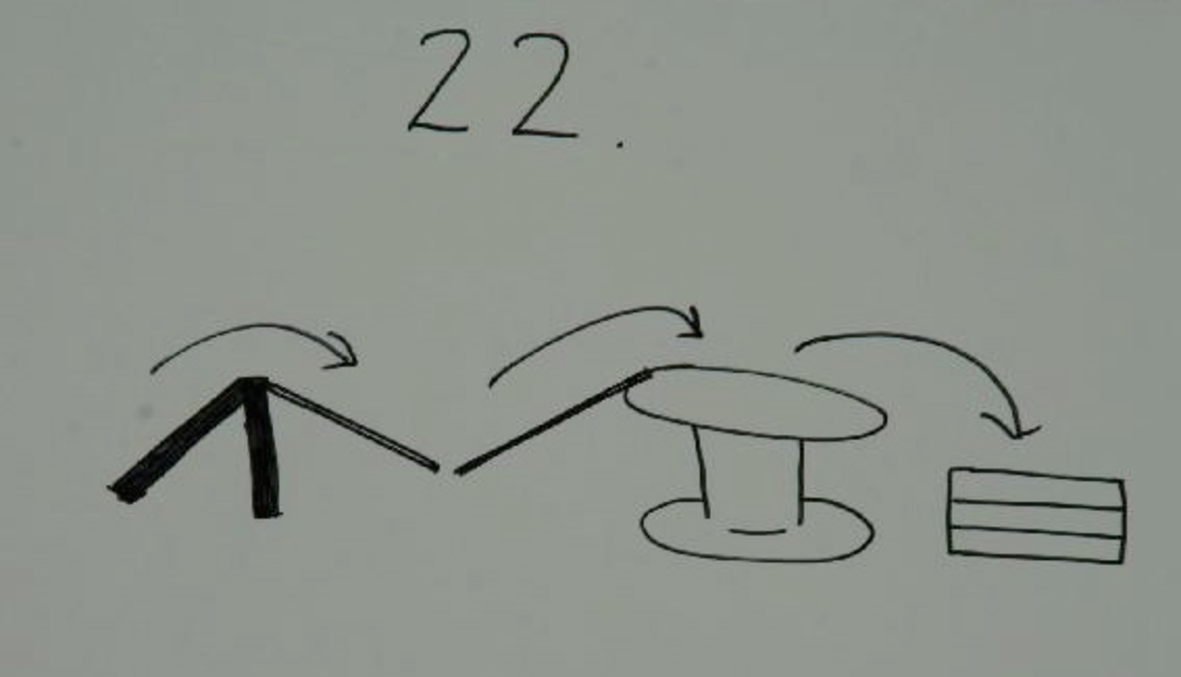
\includegraphics[scale=0.3]{trials} }\\
\hline
\end{tabular}

To make it easier to describe sections, label major obstacles with numbers and/or letters.
These should be clearly visible at a distance.
Plastic laminated cards with letters or numbers are good because they can be re-used at other competitions.

One good strategy is to label all boxes with numbers, and all beams with letters.
This makes it much easier to include section descriptions such as ``ride from Beam A to Box 6, without touching the ground.''
Section instructions should not require or prohibit a rider from using certain techniques to complete a section.
For example, the instructions must not prohibit the use of pedal grabs or bash guards in order to increase the challenge.

\subsection{Section Difficulty}
The range in difficulty of sections should correspond to the range in ability levels of the participants.
The easiest sections should be cleanable by all participants after one or two attempts, and the harder sections should require multiple attempts by the best riders.

It is highly recommended to include one or two sections that are so difficult that they may only be cleaned by one rider, or not at all.
This will help prevent ties for first place, and may also help to increase the technical standards of the sport if a rider succeeds in doing something that has never been done before.

\subsection{Assigning Difficulty Ratings to Sections \label{subsec:trials_guidelines-for-course-setters_assigning-difficulty-ratings}}
Assigning difficulty ratings to sections is optional, except if required to set section restrictions for competition categories (see section \ref{sec:trials_section-restrictions-for-competition-categories}).
However it is recommended as it helps riders plan which sections they want to attempt.
The most important responsibility when assigning difficulty ratings is to be consistent.
For this reason it is best to assign difficulty ratings after all sections have been built.
Course setters should also try not to let their own strengths and limitations at different techniques bias their judgment of score values.
This is especially important for rating sections that have similar difficulty levels but that require different skills (for example: hopping, riding narrow beams, pedal grabs, etc.).
The sections can be sorted into ``green'' (easier), ``blue'' (mid-range), and ``black'' (harder).
Each line should be marked clearly with one of these colors so that it can be seen at a distance.
If possible, the same color scheme should be shown on the rider's scoring card to make it easier for the riders to find sections of particular difficulty levels.

Two alternative methods can be used to assign ratings:

\textbf{Relative Method:}
For the purpose of grouping obstacles by difficulty, the difficulty ratings can be assigned relative to other sections in the course.
A typical course would have 25\% green lines, 50\% blue lines and 25\% black lines.

\textbf{Absolute Method:}
Experienced course setters may assign Green, Blue, and Black lines based on absolute ratings of difficulty levels.
The U-System, the open-ended difficulty rating system for unicycle trials, should be used to apply ratings.
Note that the the U-system is NOT the same as the International Unicycling Federation (IUF) Skill Levels.
Because the U-system is open-ended and based on rider consensus, description of reference obstacles is outside the scope of the IUF Rulebook.
For information on the U-System, visit www.krisholm.com/u-system.

Difficulty levels can be grouped as follows:

Green lines: U0 – U2

Blue lines: U3 – U6 

Black lines: U7 and harder

In addition to assigning Green, Blue, and Black groupings, experienced course setters may wish to label each obstacle with a U-rating.
It may be helpful to rate all obstacles first, and then use this to group the obstacles by difficulty.

\subsection{Course Planning: Location And Materials}
It is most important to make maximum use of available resources.
Prior planning and proper site selection are essential.
Expect to take at least one day to set a course for a major competition, plus time to assemble the raw building materials.

If possible, select a course location with an abundance of natural obstacles, or features that can be incorporated into human-constructed obstacles.
It cannot be overstated that is much easier to make use of what is already there, rather than constructing new obstacles.

Sections may be set on natural features such as bedrock, boulders, logs, and hill slopes, and/or constructed from stacked pallets, railings, truck tires, junkyard cars, obstacles constructed from lumber, or any other material at hand.
Often it is good to combine natural features with human-constructed obstacles.

It is highly recommended to also build a basic practice area to be set up outside of the competition area.
This can consist of a small number of random obstacles, and is important for warm-up and to reduce the temptation to ride on the course prior to the event.

Make sure that there is plenty of extra building material (tools, screws, and raw materials) on hand to repair sections damaged during the event.

\subsection{Course Design}
Sections should differ substantially from each other and test a variety of hopping and rolling techniques.
Often, it is a good idea to mentally make a list of the different techniques in trials, and design sections that test each of them separately or in combination.

The course layout is controlled mainly by the available resources.
If there are abundant natural obstacles, design sections around the most obvious natural features.

For either natural or artificial sections, a good way to maximize resources is to first construct several major structures that can be used as centerpieces, or hubs, and then design sections that center around these hubs.
For example, a car, spool, or large boulder could serve as a hub, surrounded by smaller structures that lead onto and over the hub in different ways.

Building centralized hubs rather than independent sections allows for high concentrations of sections on less building material.
Unlike conventional bike trials, it is not a problem to design overlapping sections, although sometimes it may cause delays as riders wait for their turn.
Usually a combination of hubs and independent sections is best.

It is extremely important to design sections that are durable enough that they do not break or change during the competition time period.

Overall, a course should not favor left or right handed riders, or riders with right- or left-foot-forward hopping stances.
For example, the Course Setter should include sections requiring hops to both the right and to the left.

It is best to design sections that provide challenge without undue risk.
Typically the best-designed sections include moves that test balance and precision, rather than moves that are difficult only because they are big.
For example, rather than constructing a big, basic drop or gap between easy terrain, increase the difficulty of the takeoff or landing areas by making them smaller or off-angle.
It is strongly recommended to avoid building any drops to hard, flat ground that are greater than 1.5m height.

There is no requirement that riders exit a section while in full control of their cycle.
Consequently, a well-designed section should force riders to be in control in order to finish---it should not be common for riders to fall across the finish line.
The easiest way to do this is to include at least 2 meters of easy ground between the last hard obstacle and the finish line.

\subsection{Time And Space-Saving Strategies}
If building material is extremely limited and there are very few participants, an alternative competitive strategy is to create an elimination round, instead of setting an entire course.

A small number of sections are set (as little as 1 section at a time), and riders attempt all sections.
Any rider who cannot clean an obstacle after multiple attempts is eliminated.
Then a second set of section(s) is set, and the process repeated until only one rider can clean the section(s).
This option works with minimal resources but should be regarded as a last resort.

\section{Multiple Rounds}
This new format is to be tested and report how it works during the next two years.

The competition is be formed by multiple rounds on the same course.
Each round will be managed as a single trials competition.
All other rules remain the same and each round will reset the time limit and the number of points scored.

Each round will have a time slot and there must be at least 2 hours in between each of the rounds.
Different rounds can be scheduled on different days.
The organizer must keep the course well built for all the time it is necessary.
In order to improve the next round, small changes can be made to the lines during the time between rounds.
Riders' suggestion have to be managed with attention and care, the final decision of adjusting a line is that of the main judge.
No rider may attempt any obstacle during the time in between rounds.

The sum of the results of all the rounds determines the ranking that decides which riders will compete in the final.

\section{Final}

When the competition has been completed, the top riders for male and female would compete in the final round for the championship.
The minimum number of top riders would be 6 for each male and female with the upper limit up to the host.
There should be at least 6-10 additional lines that represent the difficulty of the top riders.
Male and female finalists may have different lines depending on the overall ability of each gender.

In the finals, long lines with multiple skills can be built completely new or combined from existing lines which were used in the preliminaries.
The host should take attention that the lines for the final are close together and on a place that is good for spectators.
Depending on the used obstacles, there should be 20 - 30 minutes of competition time for each group.
Between the competition and the final should be a minimum of a 1-hour delay, or on another day.
 
\section{Tie Breaking}
A tie occurs when the competition finishes and one or more riders have completed the same number of sections.
The Course Setter should collaborate with the tied riders to create a new, ``tiebreaker section'' at an appropriate level of difficulty.
This section should be relatively long and may consist of several existing sections joined together, or an entirely new section.
The section should contain obstacles of increasing difficulty towards the exit location.

Each tied rider attempts this section and the winner is the person who rides the furthest without dabbing.
Only one attempt is allowed.
The furthest location of a rider is defined by the part of the cycle that is touching the ground (the crank, pedal, or tire), prior to dabbing.
There is no requirement for the rider to be in control.
For example, if a rider lands a drop onto their tire, but immediately dabs, their furthest point would be the location where their tire last touched prior to dabbing.
If more than one rider cleans the tiebreaker section, another tiebreaker should be conducted with a more difficult section.
